% Created 2018-03-19 Mon 11:44
\documentclass[11pt]{report}
\usepackage[utf8]{inputenc}
\usepackage[T1]{fontenc}
\usepackage{fixltx2e}
\usepackage{graphicx}
\usepackage{longtable}
\usepackage{float}
\usepackage{wrapfig}
\usepackage{rotating}
\usepackage[normalem]{ulem}
\usepackage{amsmath}
\usepackage{textcomp}
\usepackage{marvosym}
\usepackage{wasysym}
\usepackage{amssymb}
\usepackage{hyperref}
\tolerance=1000
\usepackage{minted}
\renewcommand\maketitle{}
\usepackage[margin=0.8in]{geometry}
\usepackage{amssymb,amsmath}
\usepackage{fancyhdr} %For headers and footers
\pagestyle{fancy} %For headers and footers
\fancyfoot[CE,CO]{}
\fancyhead[LE,LO]{}
\usepackage{lastpage} %For getting page x of y
\usepackage{float} %Allows the figures to be positioned and formatted nicely
\restylefloat{figure} %and this command
\usepackage{hyperref}
\hypersetup{urlcolor=blue}
\usepackage{titlesec}
\setcounter{secnumdepth}{4}
\usepackage{minted}
\setminted{frame=single,framesep=10pt}
\rfoot{\thepage\ of \pageref{LastPage}}
\usepackage[parfill]{parskip}
\usepackage{subfig}
\hypersetup{colorlinks=true,linkcolor=black, citecolor=black}
\usepackage{titlesec}
\usepackage{framed}
\usepackage{etoolbox}
\date{}
\title{\textbf{Modelling the effects of domestication in Wheat through novel computer vision techniques}}
\hypersetup{
  pdfkeywords={},
  pdfsubject={},
  pdfcreator={Emacs 25.3.1 (Org mode 8.2.10)}}
\begin{document}

\maketitle
\titleformat{\chapter}[display]
   {\normalfont\huge\bfseries}{\chaptertitlename\ \thechapter}{20pt}{\Huge}
\titlespacing*{\chapter}{0pt}{0pt}{0pt}


% Redefine the plain page style
\fancypagestyle{plain}{%
  \fancyhf{}%
  \renewcommand{\headrulewidth}{0pt}% Line at the header invisible
  \rfoot{\thepage\ of \pageref{LastPage}}
  \fancyfoot[CE,CO]{}
}

% \patchcmd{\chapter}{\thispagestyle{fancy}}{\thispagestyle{fancy}}{}{}
\thispagestyle{empty}
\renewcommand{\headrulewidth}{0pt}
\begin{center}
  \fontsize{10}{12}
  \selectfont

  \textbf{\huge Modelling the effects of domestication in Wheat through novel computer vision techniques}

  \vspace{0.3in}

  \begin{tabular}[t]{ll}
    Author: & Nathan Hughes (nah26@aber.ac.uk) \\
    Supervisor: & Dr. Wayne Aubrey (waa2@aber.ac.uk) \\
    Degree Scheme &  G401 \hspace*{0.05in}(Computer Science)\\
    \\
    \\
    Date: & \today \\
    Revision: & 0.1\\
    Status: & Draft\\
    \\
  \end{tabular}
  \\
  \vspace{0.1in}
  This report was submitted as partial fulfilment \\of a BSc degree in Computer Science (G401)
\end{center}
\clearpage
\renewcommand{\headrulewidth}{1pt}
\thispagestyle{plain}

\begin{center}
  {\LARGE\bf Declaration of originality}
\end{center}

I confirm that:

\begin{itemize}
\item{This submission is my own work, except where
    clearly indicated.}

\item{I understand that there are severe penalties for Unacceptable Academic Practice, which can lead to loss of marks or even the withholding of a degree.}

\item{I have read the regulations on Unacceptable Academic Practice from the University's Academic Quality and Records Office (AQRO) and the relevant sections of the current Student Handbook of the Department of Computer Science.}

\item{In submitting this work I understand and agree to abide by the University's regulations governing these issues.}
\end{itemize}

\vspace{2em}
Name ............................................................  \\

\vspace{1em}
Date ............................................................ \\

\vspace{1em}
\begin{center}
  {\LARGE\bf Consent to share this work}
\end{center}

By including my name below, I hereby agree to this dissertation being made available to other students and academic staff of the Aberystwyth Computer Science Department.

\vspace{2em}
Name ............................................................  \\

\vspace{1em}
Date ............................................................ \\

\clearpage
\tableofcontents
\listoftables
\listoffigures
\listoflistings
\clearpage


\chapter{Introduction, Analysis and Objectives}
\label{sec-1}

\section{Background}
\label{sec-1-1}

\section{Problem Analysis}
\label{sec-1-2}

\section{Objectives}
\label{sec-1-3}

\chapter{Method Design}
\label{sec-2}

\section{Improvements to 3D imaging software}
\label{sec-2-1}
\subsection{New Watershed Algorithm}
\label{sec-2-1-1}

In order to solve the problem of misidentified and joint seeds, from the primitive collection,
I implemented a \emph{quasi-euclidean} distance transform into the analysis pipeline \cite{Hughes2017}. This provided much better results than the previous
\emph{chessboard} transform which had been successful on more uniform datasets.

\subsubsection{Quasi-Euclidean algorithm}
\label{sec-2-1-1-1}

This algorithm measures the total euclidean distance along a set of horizontal, vertical and diagonal
line segments \cite{Pfaltz1966}.

\begin{equation}
\label{eqn:qe}
\left | x_1 - x_2 \right | + (\sqrt{2}-1), \left | x_1 - x_2 \right | >\left | y_1 - y_2 \right | (\sqrt{2}-1) \left | x_1 - x_2 \right | ,\textup{otherwise}
\end{equation}


In order to apply this to a 3D space Kleinberg's method is used  \cite{Kleinberg1997}. This allows for nearest neighbour pixels to be sorted by $k$-dimensional trees
and enabling fast distance transforms via Rosenfeld and Pfaltz's \emph{quasi-euclidean} method stated in equation:\ref{eqn:qe}.

\subsection{Code}
\label{sec-2-1-2}
\begin{listing}[H]
\begin{minted}[]{octave}
function [W] = watershedSplit3D(A)
  % Takes image stack A and splits it into stack W
  % Convert to BW
  bw = logical(A);
  % Create variable for opening and closing
  se = strel('disk', 5);
  % Minimise object missshapen-ness
  bw = imerode(bw, se);
  bw = imdilate(bw, se);
  % Fill in any left over holes
  bw = imfill(bw,4,'holes');
  % Use chessboard for distance calculation for more refined splitting
  chessboard = -bwdist(~bw, 'quasi-euclidean');
  % Modify the intensity of our bwdist to produce chessboard2
  mask = imextendedmin(chessboard, 2);
  chessboard2 = imimposemin(chessboard, mask);
  % Calculate watershed based on the modified chessboard
  Ld2 = watershed(chessboard2);
  % Take original image and add on the lines calculated for splitting
  W = A;
  W(Ld2 == 0) = 0;
end
\end{minted}
\caption{\label{lst:ws}MATLAB Watershedding function}
\end{listing}

\section{Testing of Software}
\label{sec-2-2}

\chapter{Software Design, Testing and Implementation}
\label{sec-3}

\section{Software Development Methodology}
\label{sec-3-1}

\section{Data Pipeline}
\label{sec-3-2}

\begin{center}
\begin{figure}[htb]
\centering
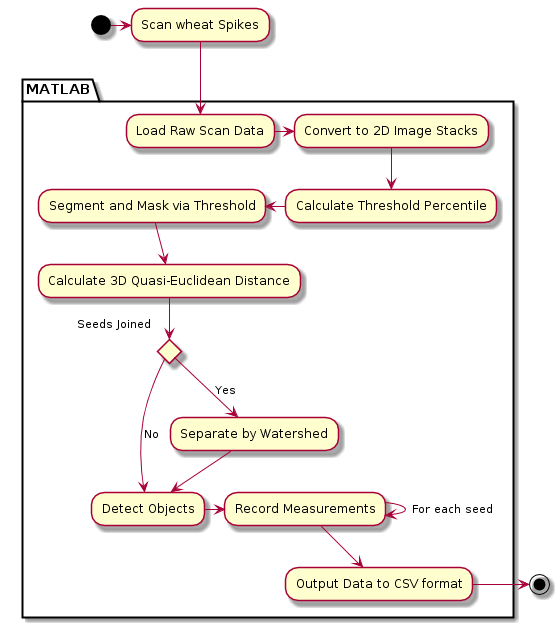
\includegraphics[width=10cm]{./images/matlab.png}
\caption{\label{fig:matlab}Image Processing Pipeline}
\end{figure}
\end{center}


\begin{center}
\begin{figure}[htb]
\centering
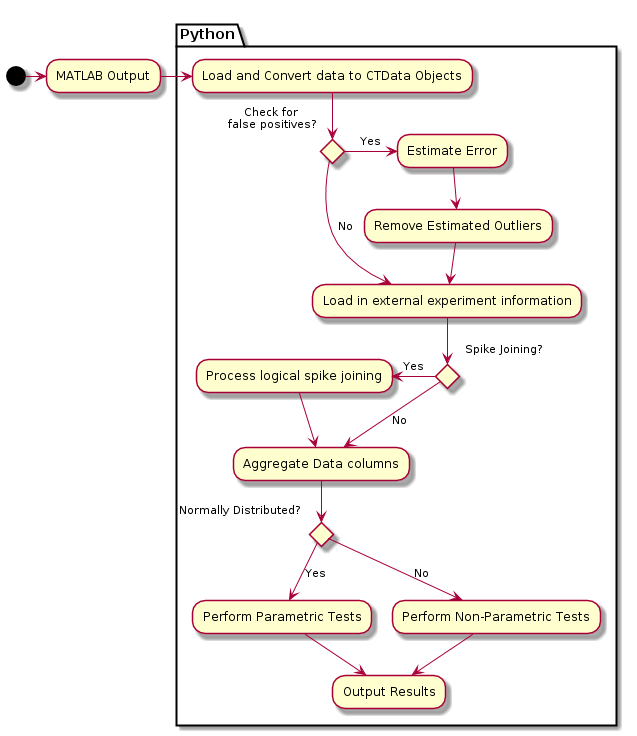
\includegraphics[width=10cm]{./images/pipeline.png}
\caption{\label{fig:pipeline}Data Pipeline and Information Flow}
\end{figure}
\end{center}

\chapter{Results}
\label{sec-4}

\section{Improved accuracy of imaging software}
\label{sec-4-1}

\subsection{Effect of enhanced watershedding algorithm}
\label{sec-4-1-1}
\begin{center}
\begin{figure}[htb]
\centering
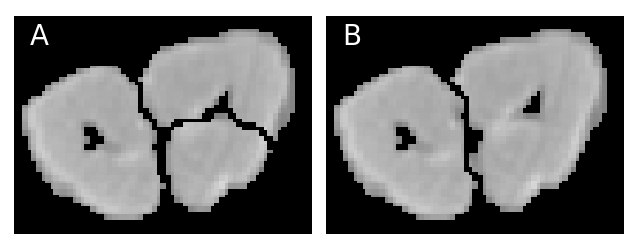
\includegraphics[width=10cm]{./images/chess_quasi.png}
\caption{\label{fig:qe}\emph{A} showing the chessboard method, \emph{B} improved quasi-euclidean method}
\end{figure}
\end{center}

\chapter{Discussion}
\label{sec-5}
\chapter{Critical Evaluation}
\label{sec-6}
\section{Organisational Methods}
\label{sec-6-1}
\section{Relevance to Degree}
\label{sec-6-2}
\section{Time Management}
\label{sec-6-3}
\section{Collaborative Work}
\label{sec-6-4}
\section{Other Issues}
\label{sec-6-5}


\clearpage
\bibliography{dissertation}
\bibliographystyle{unsrt}
% Emacs 25.3.1 (Org mode 8.2.10)
\end{document}
